
\chapter{Implementacija i korisničko sučelje}

		
		\section{Korištene tehnologije i alati}
		
Komunikacija u timu realizirana je korištenjem aplikacije MS Teams\footnote{\url{https://www.microsoft.com/hr-hr/microsoft-365/microsoft-teams}}.\newline
\indent Za izradu UML dijagrama korišten je alat Visual Paradigm Online\footnote{\url{https://online.visual-paradigm.com}}, a kao sustav za upravljanje izvornim kodom Git\footnote{\url{https://git-scm.com}}, a udaljeni repozitorij projekta je dostupan na web platformi GitLab\footnote{\url{https://gitlab.com/}}.\newline
\indent Kao razvojno okruženje korišten je Visual Studio  Code\footnote{\url{https://code.visualstudio.com/}}, integrirano razvojno okruženje (kratica IDE) tvrtke Microsoft. Koristi se prvenstveno za razvoj računalnih programa za operacijski sustav Windows, kao i za web-stranice, web-aplikacjie, mobilne aplikacije i web-usluge. Visual studio za razvoj softvera koristi Microsoftove platforme kao što su Windows API, Windows Forms, Windows Presentation Foundation, Windows Store i Microsoft Silverlight.\newline
\indent Baza podataka se nalazi na pgAdmin 4 platformi\footnote{\url{https://www.pgadmin.org/}}.\\
			
			\eject 
		
	
		\section{Ispitivanje programskog rješenja}
	
			
			\subsection{Ispitivanje komponenti}
			{U okviru paketa \textbf{Mocha} i \textbf{Chai} proveden je unit testing. Testovi su provedeni nad nekim funkcionalnostima razreda Grupa, Kamp, Sudionik, MailSender i Osoba.\\\\}
			
			\textbf{\large Testovi kamp klase}
			\begin{verbatim}
			const assert = require('assert');
			const Kamp = require('../models/Kamp');
			
			describe('Kamp Test', () => {
				it('treba vratiti undefined jer nema kampa', () => {
					assert.equal(undefined, Kamp.provjeriImaLiKampa().pocetak);
				});
				
				it('treba vratiti 2',async () => {
					let kamp = new Kamp("2021-01-14T18:47", 2, []);
					await kamp.persist();
					let result = await Kamp.provjeriImaLiKampa();
					assert.equal(result.trajanje, 2);
					await Kamp.otkaziKamp();
				});
			});
			\end{verbatim}
		
			\newpage
			
			
			\textbf{\large Testovi grupa}
			\begin{verbatim}
			const assert = require('assert');
			const Grupa = require('../models/Grupa');
			
			describe('Grupa Test', () => {
				it('treba vratiti naziv grupe', async () => {
					let grupa = new Grupa("grupa 1")
					await grupa.persist();
					let result = await Grupa.fetchAllGroups();
					assert.equal(result[0].naziv, "grupa 1");
				});
			});
			\end{verbatim}
			
			
			\textbf{\large Testovi pošiljatelja mailova}
			\begin{verbatim}
			const assert = require('assert');
			const MailSender = require('../models/MailSender');
			
			describe('Mail Sender Test', () => {
				
				it('treba vratiti poruku prihvaćanja', () => {
					let mailOptions = MailSender.send("korisnik@random.com", "krandom", "accepted");
					assert.equal(mailOptions.subject, 'Čestitamo! Primljeni ste u naš kamp!');
				});
				
				it('treba vratiti poruku odbijanja', () => {
					let mailOptions = MailSender.send("korisnik2@random.com", "krandom2", "denied");
					assert.equal(mailOptions.subject, 'Vaš zahtjev je obijen');
				});
			});
			\end{verbatim}
			
			\newpage
			
			\textbf{\large Test za random raspored sudionika u grupe}
			\begin{verbatim}
			const expect = require('chai').expect;
			const assert = require('assert');
			
			
			describe('Shuffle Test', () => {
				
				it('liste trebaju imati ispremiješane elemente',async () => {
					let array = [1, 2, 1, 2, 3, 3];
					let arrayShuffled = [1, 2, 1, 2, 3, 3];
					arrayShuffled = shuffle(arrayShuffled);
					console.log(array);
					console.log(arrayShuffled);
					assert.notStrictEqual(array, arrayShuffled);
				});
				
				it('liste trebaju imati iste elemente', () => {
					let array = [1, 2, 1, 2, 3, 3];
					let arrayShuffled = [1, 2, 1, 2, 3, 3];
					arrayShuffled = shuffle(arrayShuffled);
					expect(array).to.have.same.members(arrayShuffled);
				});
			});
			
			function shuffle(array) {
				for (var i = array.length - 1; i > 0; i--) {
					var j = Math.floor(Math.random() * (i + 1));
					var temp = array[i];
					array[i] = array[j];
					array[j] = temp;
				}
				return array
			}
			\end{verbatim}
		
			\newpage
			
			\textbf{\large Screenshot pokretanja i uspjeha testova}
			
			\begin{figure}[h]
				\centering
				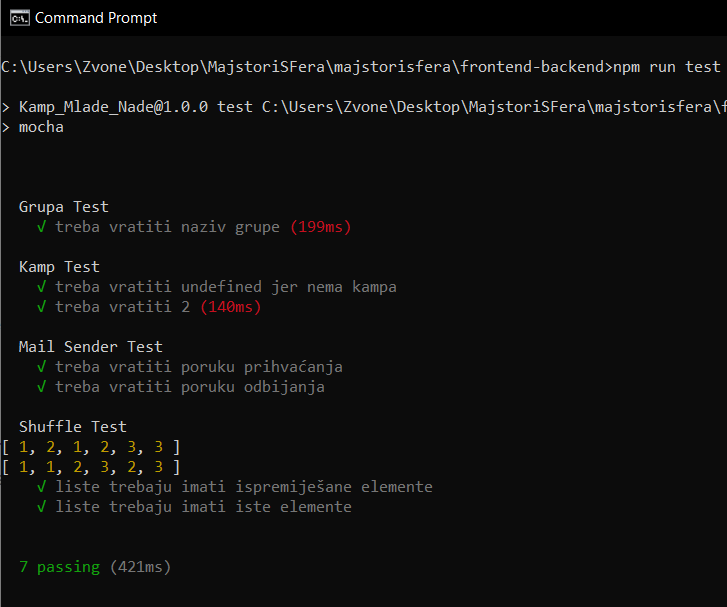
\includegraphics[scale=1.0]{testovi}
				\caption{Pokrenuti testovi}
			\end{figure}
			
			\newpage
			
			\subsection{Ispitivanje sustava}
			
			{Pomoću radnog okvira Selenium provedeno je ispitivanje funkcionalnosti organizacije kampa i organizacije prijave za kamp, prijave osobe na kamp, potvrde prijave od strane organizatora te registracije korisnika. Za izradu ispitnih slučajeva korišten je alat Selenium IDE.\\ }
			
			\textbf{Ispitni slučaj 1: Organizacija kampa i prijava za kamp\\}
				\indent\textbf{Ulaz:}
					\begin{packed_item}
						\item {Prijava kao organizator.}
						\item {Organiziranje kampa u određeno vrijeme.}
						\item {Organiziranje prijava u određeno vrijeme.}
					\end{packed_item}
			
				\textbf{Očekivani rezultat:}
					\begin{packed_item}
						\item {Na početnoj stranici ispisano je vrijeme početka i vrijeme trajanja kampa.}
					\end{packed_item}
			
				{\textbf{Rezultat:} Očekivani rezultat je zadovoljen. Aplikacija je prošla test.}
			
			\begin{figure}[h]
				\centering
				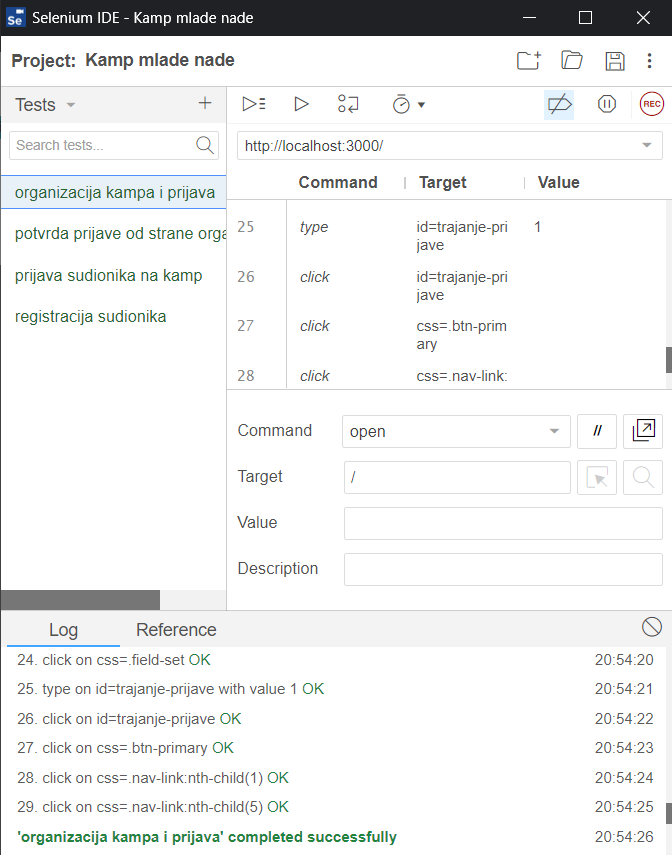
\includegraphics[scale=0.6]{organizacijaKampaIPrijava}
				\caption{Organizacija kampa i prijava}
			\end{figure}
			
			\clearpage
			
			\textbf{Ispitni slučaj 2: Prijava sudionika na kamp\\}
				\indent\textbf{Ulaz:}
					\begin{itemize}
						\item {Unos podataka korisnika u sklopu prijave za sudionika na kampu.}	
					\end{itemize}
				
				\textbf{Očekivani rezultat:}
					\begin{itemize}
						\item {Prijava evidentirana u bazi i samim tim se prikazuje organizatoru na stranici sa prijavama.}
					\end{itemize}
			
				{\textbf{Rezultat:} Očekivani rezultat je zadovoljen. Aplikacija je prošla test.\\}
			
			\begin{figure}[h]
				\centering
				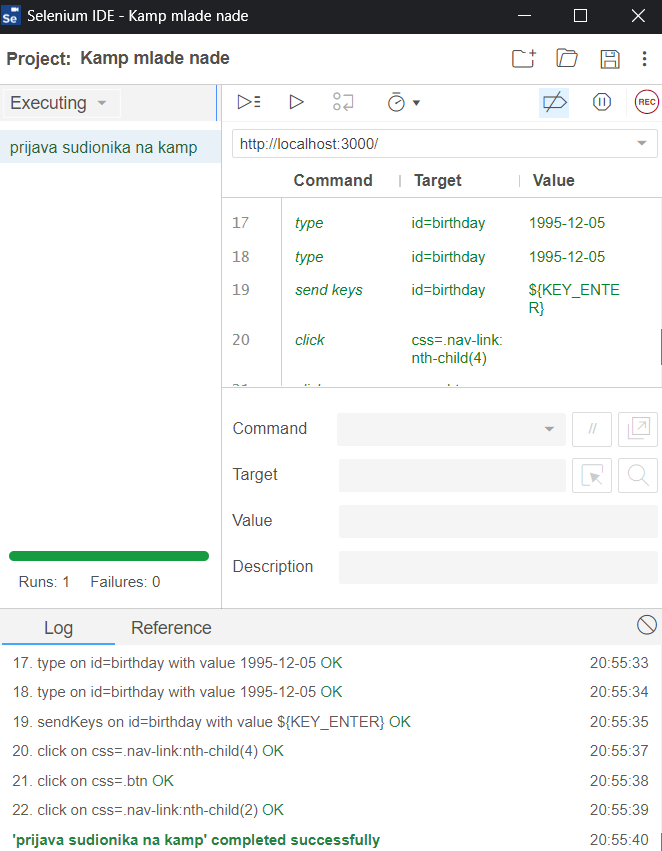
\includegraphics[scale=0.7]{prijavaSudionikaNaKamp}
				\caption{Organizacija kampa i prijava}
			\end{figure}
			
			\clearpage
			
			\textbf{Ispitni slučaj 3: Potvrda prijave od strane organizatora\\}
				\indent\textbf{Ulaz:}
					\begin{itemize}
						\item {Prijava korisnika u kojoj organizator vidi njegove podatke}
						\item {Odabir hoće li prihvatiti ili odbiti prijavu.}
					\end{itemize}
			
				\textbf{Očekivani rezultat:}
					\begin{itemize}
						\item {Na stranici na kojoj organizator inače može vidjeti prijave više nema prijave koja je potvrđena.}
						\item {Korisniku je poslan mail sa linkom i korisničkim imenom za registraciju.}
					\end{itemize}
			
				{\textbf{Rezultat:} Očekivani rezultat je zadovoljen. Aplikacija je prošla test.\\}
			
			\begin{figure}[h]
				\centering
				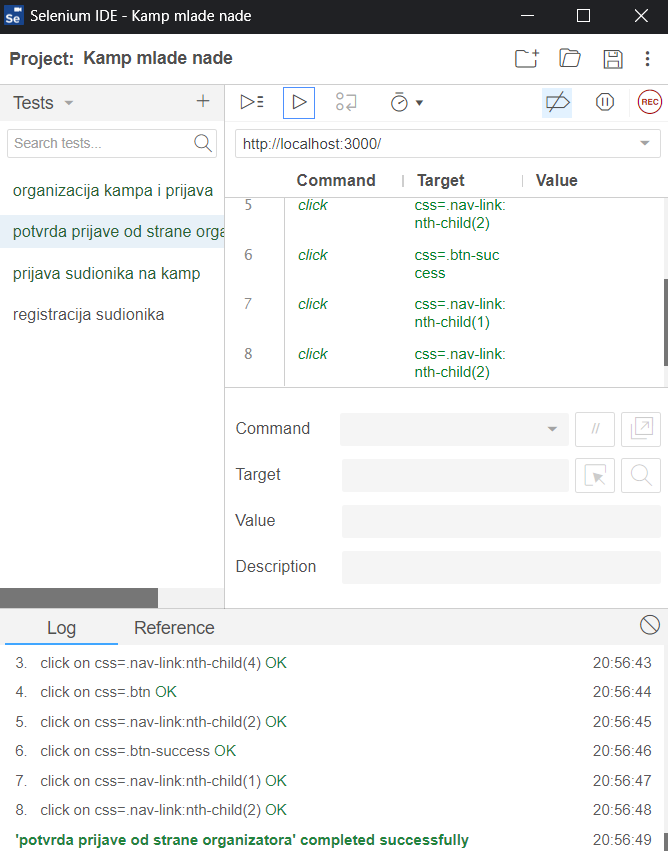
\includegraphics[scale=0.7]{potvrdaPrijaveOdStraneOrganizatora}
				\caption{Potvrda prijave od strane organizatora}
			\end{figure}

			
			\clearpage
			
			\textbf{Ispitni slučaj 4: Registracija sudionika\\}
			\indent\textbf{Ulaz:}
				\begin{itemize}
					\item {Web lokacija za kompletiranje registracije.}
					\item {Korisničko ime za registraciju.}
				\end{itemize}
			
			\textbf{Očekivani rezultat:}
				\begin{itemize}
					\item {Sudionik kampa uspješno se ulogirao.}
					\item {Sudionik kampa može vidjeti svoje korisničko ime u gornjem desnom kutu.}
					\item {Sudioniku se otvaraju opcije koje na web stranici ima svaki sudionik.}
				\end{itemize}
			
			{\textbf{Rezultat:} Očekivani rezultat je zadovoljen. Aplikacija je prošla test.\\}
			
			\begin{figure}[h]
				\centering
				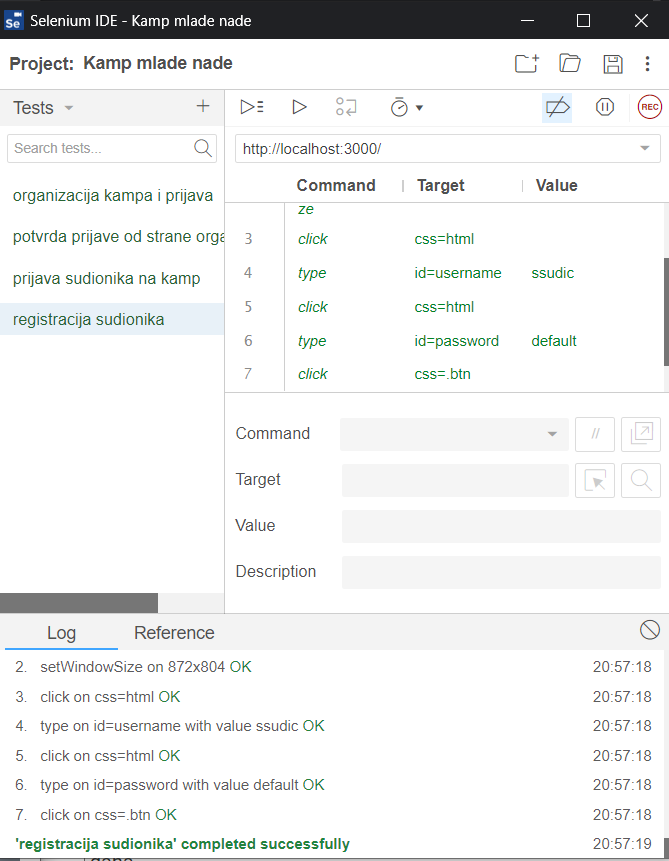
\includegraphics[scale=0.7]{registracijaSudionika}
				\caption{Registracija sudionika}
			\end{figure}
			
			\clearpage
			
			\textbf{Ispitni slučaj 5: Pokušaj organiziranja prijave nakon početka kampa\\}
			\indent\textbf{Ulaz:}
			\begin{itemize}
				\item {Datum i vrijeme početka kampa}
				\item {Odabir početka prijava u korisničkom sučelju.}
			\end{itemize}
			
			\textbf{Očekivani rezultat:}
			\begin{itemize}
				\item {Organiziranje prijave se odbija uz prikladnu poruku.}
				\item {Organizator je preusmjeren na početnu stranicu}
			\end{itemize}
			
			{\textbf{Rezultat:} Očekivani rezultat nije zadovoljen. Pokušajem organiziranja prijave nakon početka kampa događa se ReferenceError. Aplikacija nije prošla test.\\}
			
			\begin{figure}[h]
				\centering
				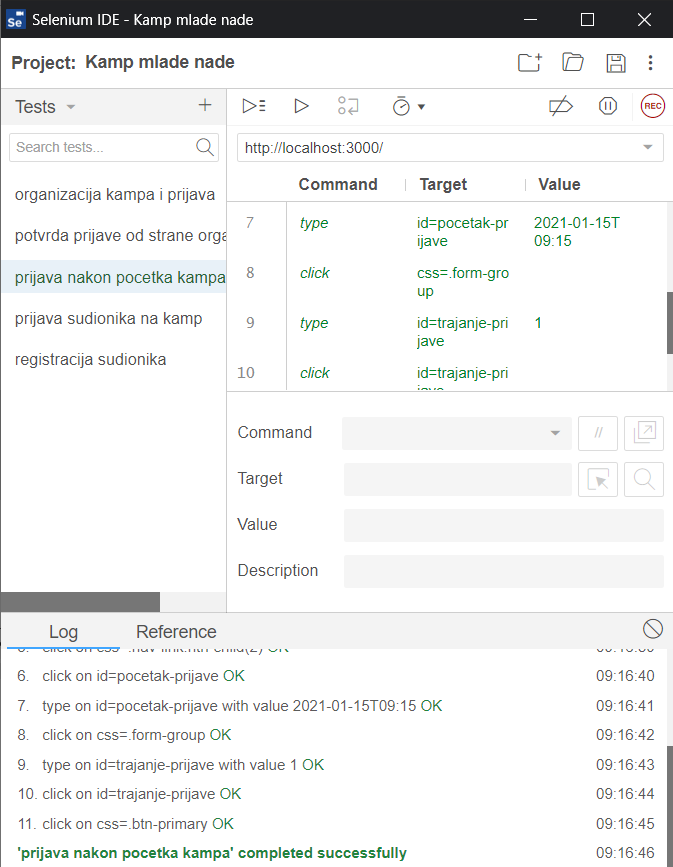
\includegraphics[scale=0.7]{prijavaNakonPocetka}
				\caption{Organiziranje prijave nakon početka kampa}
			\end{figure}

			
			\eject 
		
		
		\section{Dijagram razmještaja}
			
			Dijagrami razmještaja prikazuju računalne resurse potrebne za ispravno funkcioniranje sustava te njihove međusobne odnose: stvarne uređaje, komponente programske potpore koje se na njima izvršavaju i veze između njih. Dijagram razmještaja je statički strukturni UML-dijagram.\newline
			\indent Sustav je temeljen na arhitekturi \textit{klijent-poslužitelj}. Na poslužiteljskom računalu nalaze se web poslužitelj (na kojem se nalazi web aplikacija) i poslužitelj baze podataka (na kojem se nalazi baza podataka). Web poslužitelj i poslužitelj baze podataka su u vezi ovisnosti, točnije promjene na web poslužitelju uzrokuju promjene u bazi podataka. Na klijentskom se računalu nalazi web preglednik putem kojeg se pristupa web poslužitelju, odnosno web aplikaciji. Komunikacija između klijentskog i poslužiteljskog računala odvija se preko HTTP veze.\\\\
			
			\begin{figure}[htb]
				\centering
				\includegraphics[scale=0.7]{dijagrami/dijagramRazmještaja.PNG}
				\caption{Dijagram razmještaja}
				\label{fig: dijagram razmještaja}
			\end{figure}
			
			\eject 
		
		\section{Upute za puštanje u pogon}
		
			\subsection{Instalacija Git-a}
				Potrebno je instalirati Git korisničko sučelje prema uputama na stranici\footnote{\url{https://git-scm.com/book/en/v2/Getting-Started-Installing-Git}} i na računalu kreirati novu mapu za aplikaciju. Nakon instalacije potrebno je otvoriti \textit{Git Bash} i pozicionirati se u direktorij namijenjen za datoteke aplikacije. To se može učiniti tako da se desnim klikom na željenu mapu odabere opcija \textit{Git Bash Here}. Sljedeći korak je prijava ili registracija na sustav Gitlab putem internet stranice i postavljanje podataka o korisničkom računu na lokalni Git repozitorij. To se obavlja upisivanjem sljedećih naredbi u Git Bash:
					\begin{itemize}
						\item \textit{\textbf{git config user.email}} \textit{email}
						\item \textit{\textbf{git config user.name}} \textit{username}
					\end{itemize}
				U mapu je potrebno klonirati projekt odabirom opcije \textit{Clone} u gitlab repozitoriju te kopirati link ispod oznake \textit{Clone with HTTPS}. U Git Bash je potrebno upisati \textbf{\textit{git clone}} \textit{link}. Kod projekta je sada praćen u lokalnom Git repozitoriju.\\
				
				
			\subsection{Instalacija Heroku CLI-a}
				Heroku sučelje naredbenog retka (CLI) olakšava izradu i upravljanje Heroku aplikacijama izravno iz terminala. To je bitan dio upotrebe Herokua. Potrebno je preuzeti instalacijski paket\footnote{\url{https://devcenter.heroku.com/articles/heroku-cli}} minimalne verzije 7.0.x., pokrenuti instalacijski paket i slijediti upute na ekranu. Nakon instalacije potrebno je postaviti varijable okruženja sljedećim putem: \textit{Control Panel - System and Security - System - Advancded System Settings}. Otvorit će se prozor \textit{System properties} te je na kartici textit{Advanced} potrebno pritisnuti gumb \textit{Environment Variables}. U prozoru \textit{Environment Variables} u sekciji \textit{User Variables} potrebno je odabrati \textit{Path} i kliknuti gumb \textit{Edit}. U prozoru \textit{Edit environment variable} odabrati \textit{New} te upisati putanju do bin datoteke u folderu heroku, koja se najčešće nalazi u \textit{C://Program Files}. Ako je instalacija uspješna, u terminalu je moguće
				pokrenuti \textit{heroku -v} što će rezultirati prikazom verzije.\\
				
				
			\subsection{Kreiranje Heroku udaljenog repozitorija}
				Prvi je korak registracija i prijava u sustav Heroku. Nakon toga, potrebno je otvoriti terminal i pozicionirati se u git lokalni repozitorij, odnosno mapu kreiranu za projekt. Sljedeći korak je pokretanje naredbe \textbf{\textit{heroku login}} i nakon toga \textbf{\textit{heroku plugins:install java}}. Sljedeća naredba koju je potrebno pokrenuti je \textbf{\textit{heroku create}} u naredbenom retku (terminalu). Ta naredba stvara novu, praznu aplikaciju na Heroku poslužitelju povezanu s Git repozitorijem. Poželjno je nakon toga pokrenti naredbu \textbf{\textit{git remote -v}} što će rezultirati potvrdom da je udaljeni repozitorij pod imenom \textit{heroku} postavljen u aplikaciji.\newline
				\indent Potrebno je kreirati dvije aplikacije na Herokuu: jednu za backend i jednu za frontend. Jedna aplikacija je jedan poslužitelj.\\
				
				
			\subsection{Postavljanje baze podataka}
				Za postavljanje baze podataka potrebno je u kartici \textit{Resources} u postavkama aplikacije dodati \textit{Heroku Postgres} dodatak. Nakon ovog koraka na serveru će se konfigurirati prazna baza podataka. U kartici \textit{Settings} na postavkama baze podataka potrebno je odabrati opciju \textit{View Credentials}. Tada dobivamo podatke za spajanje na bazu koji su potrebni za konfiguraciju backenda.\\
				
				
			\subsection{Postavljanje backenda aplikacije na Heroku poslužitelj}
				Prije postavljanja backenda na poslužitelj potrebno je konfigurirati podatke za spajanje na bazu. U datoteci \textit{application.properties} unutar projekta potrebno je upisati podatke dobivene na sučelju Heroku. Nakon konfiguracije konekcije, potrebno je pokrenuti naredbu \textbf{\textit{maven install}}. Time će se izgraditi aplikacija. Unutar target direktorija unutar projekta kreirat će se \textit{.war} datoteka. Tu datoteku potrebno je prenijeti na Heroku poslužitelj.\newline
				\indent Koristeći naredbeni redak potrebno je postaviti se u direktorij projekta te pokrenuti naredbu \textbf{\textit{heroku war:deploy}} \textit{ime war datoteke} \textbf{\textit{–app}} \textit{naziv aplikacije kreirane na Heroku}. Nakon toga će na Heroku poslužitelj biti postavljen backend
				aplikacije.\\
				
				
			\subsection{Postavljanje frontenda aplikacije na Heroku poslužitelj}
				Nakon inicijalizacije udaljenog repozitorija na heroku, potrebno je pokrenuti naredbu \textbf{\textit{npm install}} za instalaciju svih paketa potrebnih \textit{node.j}-u.\newline
				\indent Da bi frontend aplikacije bio postavljen na Heroku poslužitelj, izvede se naredba
				\textbf{\textit{git push heroku master}} koja \textit{pusha} kod iz lokalnog repozitorija grane master na heroku udaljeni repozitorij. Ovu naredbu potrebno je pokrenuti svaki puta kada se želi postaviti novija verzija aplikacije na Heroku.
				\begin{figure}[htb]
					\centering
					
\includegraphics[scale=0.6]{slike/herokuPush.PNG}
					\caption{Postavljanje nove verzije aplikacije na Heroku}
					\label{fig: heroku}
				\end{figure}
			
				\indent Na kraju, naredba \textit{\textbf{heroku open}} služi za pokretanje aplikacije u pretpostavljenom pretraživaču.
			
			
			\eject 